\section{Dataset and preprocessing}
\label{sec:dataset}
The dataset used in this project is called \textit{Flowers-299} and is published on \href{https://www.kaggle.com/bogdancretu/flower299}{kaggle} unter the \textit{CC0: Public Domain} license \cite{data}.
It contains sorted images of 299 different flower species and for each species there are between 222 and 483 images which vary in size.
From among these we choose eleven species to include in our project.
This number of species was chosen to limit the scale of the project with regards to the limited time and computing resources available to us.
While selecting the eleven species we tried to include flowers that are more easily distinguishable for the human eye, as well as some which look quite similar.

We use the \texttt{Python Image Library Pillow} \cite{pillow} to load the images and start by inspecting the distribution of their lengths and widths which can be seen in \autoref{fig:sizes}.
In order to use the images as the input for a neural network all the images must be of the same size. 
Therefore, we have to resize all the images to the same size.
We choose $200\times200$ pixels for this, as most images have a bigger native size, no image artifacts will be created using this image size (which could happen by upscaling images).
A resized example image of each of the chosen flower species can be seen in \autoref{fig:images}.
\begin{figure}
    \centering    
    \begin{subfigure}{0.49\textwidth}
        \centering
        \includegraphics[width=0.99\textwidth]{../data/width_vs_height.pdf}
        \caption{The distribution of the lengths and widths of the images.}
        \label{fig:sizes}
    \end{subfigure}
    \hfill
    \begin{subfigure}{0.49\textwidth}
        \centering
        \includegraphics[width=0.99\textwidth]{../data/ratio_hist_limits.pdf}
        \caption{Histogram of the aspect ratios of the images.}
        \label{fig:ratio}
    \end{subfigure}
    \caption{Most of the images' size exceeds $200\times200$ pixels. 
        Additionally images with an aspect ratio smaller than 0.55 or bigger than 1.82 are discarded to avoid heavily clinched or stretched images after resizing. }
\end{figure}
\begin{figure}
    \centering
    \begin{subfigure}{0.24\textwidth}
        \centering
        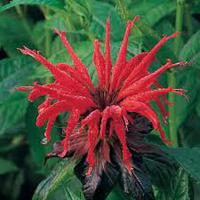
\includegraphics[width=0.9\textwidth]{../example_images/BeeBalm.jpg}
        \caption{Bee Balm.}
    \end{subfigure}
    \vspace{0.07cm}
    \begin{subfigure}{0.24\textwidth}
        \centering
        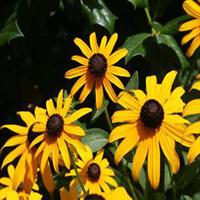
\includegraphics[width=0.9\textwidth]{../example_images/Black-eyedSusan.jpg}
        \caption{Black-eyed Susan.}
    \end{subfigure}
    \vspace{0.07cm}
    \begin{subfigure}{0.24\textwidth}
        \centering
        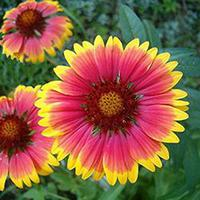
\includegraphics[width=0.9\textwidth]{../example_images/BlanketFlower.jpg}
        \caption{Blanket Flower.}
    \end{subfigure}
    \vspace{0.07cm}
    \begin{subfigure}{0.24\textwidth}
        \centering
        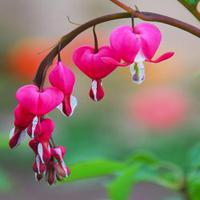
\includegraphics[width=0.9\textwidth]{../example_images/BleedingHeart.jpg}
        \caption{Bleeding Heart.}
    \end{subfigure}
    \vspace{0.07cm}
    \begin{subfigure}{0.24\textwidth}
        \centering
        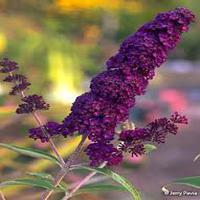
\includegraphics[width=0.9\textwidth]{../example_images/ButterflyBush.jpg}
        \caption{Butterfly Bush.}
    \end{subfigure}
    \vspace{0.07cm}
    \begin{subfigure}{0.24\textwidth}
        \centering
        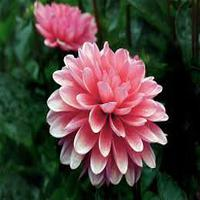
\includegraphics[width=0.9\textwidth]{../example_images/Dahlia.jpg}
        \caption{Dahlia.}
    \end{subfigure}
    \vspace{0.07cm}
    \begin{subfigure}{0.24\textwidth}
        \centering
        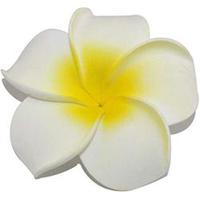
\includegraphics[width=0.9\textwidth]{../example_images/FrangipaniFlower.jpg}
        \caption{Frangipani Flower.}
    \end{subfigure}
    \vspace{0.07cm}
    \begin{subfigure}{0.24\textwidth}
        \centering
        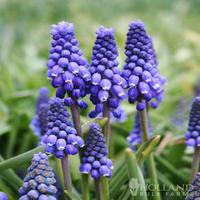
\includegraphics[width=0.9\textwidth]{../example_images/GrapeHyacinth.jpg}
        \caption{Grape Hyacinth.}
    \end{subfigure}
    \vspace{0.07cm}
    \begin{subfigure}{0.24\textwidth}
        \centering
        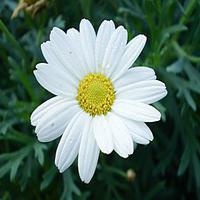
\includegraphics[width=0.9\textwidth]{../example_images/MargueriteDaisy.jpg}
        \caption{Marguerite Daisy.}
    \end{subfigure}
    \begin{subfigure}{0.24\textwidth}
        \centering
        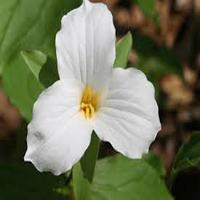
\includegraphics[width=0.9\textwidth]{../example_images/Trillium.jpg}
        \caption{Trillium.}
    \end{subfigure}
    \begin{subfigure}{0.24\textwidth}
        \centering
        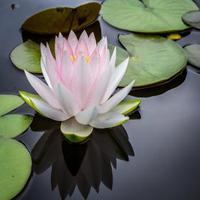
\includegraphics[width=0.9\textwidth]{../example_images/Waterlilies.jpg}
        \caption{Waterlilies.}
    \end{subfigure}
    \caption{Examples of each of the eleven flower species used. The images are resized to a resolution of $200\times200$ pixels.}
    \label{fig:images}
\end{figure}

Another point to consider is, that some images might have very different widths and heights.
This would lead to such images being heavily clinched or stretched along one axis which would greatly alter the form of the flower(s) in the image and potentially force the neural network 
to learn image features that are not representative of flowers of its species.
For this reason we look at the aspect ratios of the images in \autoref{fig:ratio} and decide to discard images with an aspect ratio smaller than 0.55 or bigger than $\sfrac{1}{0.55} = 1.82$. 

After this pre-selection the number of images for each of the flower species still varies.
To avoid a bias towards over-represented species, we only use the first 334 images of each species from here on out.
As a final preprocessing step, we split $\SI{15}{\percent}$ of the images into a test set (and $\SI{85}{\percent}$ as train set) that is not used until the final evaluation of the results.
Finally we save both sets in \texttt{hdf5}-files to speed up loading times.
All the steps described in this section are performed in the \texttt{preprocessing.ipynb} Jupyter-notebook.